\documentclass[size=a4, parskip=half, titlepage=false, toc=flat, toc=bib, 12pt]{scrartcl}

\setuptoc{toc}{leveldown}

% Ajuste de las líneas y párrafos
\linespread{1.2}
\setlength{\parindent}{0pt}
\setlength{\parskip}{12pt}

% Español
\usepackage[spanish, es-tabla]{babel}

% Matemáticas
\usepackage{amsmath}
\usepackage{amsthm}

% Links
%\usepackage{hyperref}

% Fuentes
\usepackage{newpxtext,newpxmath}
\usepackage[scale=.9]{FiraMono}
\usepackage{FiraSans}
\usepackage[T1]{fontenc}

\defaultfontfeatures{Ligatures=TeX,Numbers=Lining}
\usepackage[activate={true,nocompatibility},final,tracking=true,factor=1100,stretch=10,shrink=10]{microtype}
\SetTracking{encoding={*}, shape=sc}{0}

\usepackage{graphicx}
\usepackage{float}

% Mejores tablas
\usepackage{booktabs}

\usepackage{adjustbox}

% COLORES

\usepackage{xcolor}

\definecolor{verde}{HTML}{007D51}
\definecolor{esmeralda}{HTML}{045D56}
\definecolor{salmon}{HTML}{FF6859}
\definecolor{amarillo}{HTML}{FFAC12}
\definecolor{morado}{HTML}{A932FF}
\definecolor{azul}{HTML}{0082FB}
\definecolor{error}{HTML}{b00020}

% ENTORNOS
\usepackage[skins, listings, theorems]{tcolorbox}

\newtcolorbox{recuerda}{
  enhanced,
%  sharp corners,
  frame hidden,
  colback=black!10,
	lefttitle=0pt,
  coltitle=black,
  fonttitle=\bfseries\sffamily\scshape,
  titlerule=0.8mm,
  titlerule style=black,
  title=\raisebox{-0.6ex}{\small RECUERDA}
}

\newtcolorbox{nota}{
  enhanced,
%  sharp corners,
  frame hidden,
  colback=black!10,
	lefttitle=0pt,
  coltitle=black,
  fonttitle=\bfseries\sffamily\scshape,
  titlerule=0.8mm,
  titlerule style=black,
  title=\raisebox{-0.6ex}{\small NOTA}
}

\newtcolorbox{error}{
  enhanced,
%  sharp corners,
  frame hidden,
  colback=error!10,
	lefttitle=0pt,
  coltitle=error,
  fonttitle=\bfseries\sffamily\scshape,
  titlerule=0.8mm,
  titlerule style=error,
  title=\raisebox{-0.6ex}{\small ERROR}
}

\newtcblisting{shell}{
  enhanced,
  colback=black!10,
  colupper=black,
  frame hidden,
  opacityback=0,
  coltitle=black,
  fonttitle=\bfseries\sffamily\scshape,
  %titlerule=0.8mm,
  %titlerule style=black,
  %title=Consola,
  listing only,
  listing options={
    style=tcblatex,
    language=sh,
    breaklines=true,
    postbreak=\mbox{\textcolor{black}{$\hookrightarrow$}\space},
    emph={jmml@UbuntuServer, jmml@CentOS},
    emphstyle={\bfseries},
  },
}

\newtcbtheorem[number within=section]{teor}{\small TEOREMA}{
  enhanced,
  sharp corners,
  frame hidden,
  colback=white,
  coltitle=black,
  fonttitle=\bfseries\sffamily,
  %separator sign=\raisebox{-0.65ex}{\Large\MI\symbol{58828}},
  description font=\itshape
}{teor}

\newtcbtheorem[number within=section]{prop}{\small PROPOSICIÓN}{
  enhanced,
  sharp corners,
  frame hidden,
  colback=white,
  coltitle=black,
  fonttitle=\bfseries\sffamily,
  %separator sign=\raisebox{-0.65ex}{\Large\MI\symbol{58828}},
  description font=\itshape
}{prop}

\newtcbtheorem[number within=section]{cor}{\small COROLARIO}{
  enhanced,
  sharp corners,
  frame hidden,
  colback=white,
  coltitle=black,
  fonttitle=\bfseries\sffamily,
  %separator sign=\raisebox{-0.65ex}{\Large\MI\symbol{58828}},
  description font=\itshape
}{cor}

\newtcbtheorem[number within=section]{defi}{\small DEFINICIÓN}{
  enhanced,
  sharp corners,
  frame hidden,
  colback=white,
  coltitle=black,
  fonttitle=\bfseries\sffamily,
  %separator sign=\raisebox{-0.65ex}{\Large\MI\symbol{58828}},
  description font=\itshape
}{defi}

\newtcbtheorem{ejer}{\small EJERCICIO}{
  enhanced,
  sharp corners,
  frame hidden,
  left=0mm,
  right=0mm,
  colback=white,
  coltitle=black,
  fonttitle=\bfseries\sffamily,
  %separator sign=\raisebox{-0.65ex}{\Large\MI\symbol{58828}},
  description font=\itshape,
  nameref/.style={},
}{ejer}

% CÓDIGO
\usepackage{listings}

% CABECERAS
\pagestyle{headings}
\setkomafont{pageheadfoot}{\normalfont\normalcolor\sffamily\small}
\setkomafont{pagenumber}{\normalfont\sffamily}

% ALGORITMOS
\usepackage[vlined,linesnumbered]{algorithm2e}

% Formato de los pies de figura
\setkomafont{captionlabel}{\scshape}
\SetAlCapFnt{\normalfont\scshape}
\SetAlgorithmName{Algoritmo}{Algoritmo}{Lista de algoritmos}

% BIBLIOGRAFÍA
%\usepackage[sorting=none]{biblatex}
%\addbibresource{bibliografia.bib}

\begin{document}

\renewcommand{\proofname}{\normalfont\sffamily\bfseries\small DEMOSTRACIÓN}

\title{Proyecto final\\
ShapeContext}
\subject{Visión por computador}
\author{Johanna Capote Robayna\\
    Guillermo Galindo Ortuño\\
    5 del Doble Grado en Informática y Matemáticas\\
    Grupo A}
\date{}
\publishers{\vspace{2cm}
\includegraphics[height=2.5cm]{UGR}\vspace{1cm}}
\maketitle

\newpage

\tableofcontents
\newpage

\section{Introducción}
En este proyecto vamos a implementar el descriptor \textit{ShapeContext}, presentado por Serge Belongie and Jitendra Malik en el paper <<Matching with Shape Contexts>> en el año 2000.

La principal idea del este algoritmo se basa construir un histograma basado en puntos en el sistema de coordenadas polares. Para cada punto, se obtiene la distancia y los ángulos euclidianos con respecto a otros puntos, se normalizan y se representa en las regiones del mapa el número de puntos de cada registro.

\begin{center}
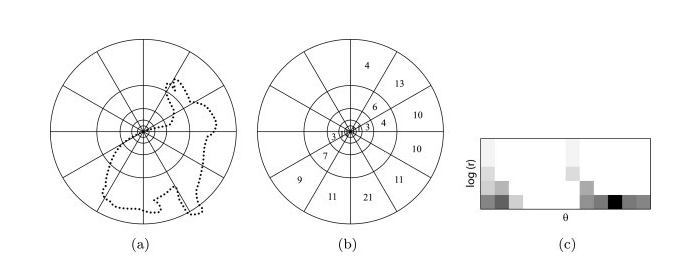
\includegraphics[height=6cm]{./img/intro}
\end{center}

Añadir información de que su utiliza principalmente para reconomiento de simbolos etc, y de sobre que lo vamos a probar etc.

\newpage

\section{Implementación}
Para implementar este algoritmo, se ha declarado una clase \verb|ShapeContext|. En el constructor declaramos los parámetros que determinan las regiones en las que se dividiremos la imagen. Es decir, el radio del circulo interior (\verb|r_inner|), el radio del último circulo exterior (\verb|r_outer|), el número de círculos concentricos (\verb|nbins_r|) y el número de regiones en las que se divide los círculos (\verb|nbins_theta|).

\begin{verbatim}
    self.nbins_r = 5
    self.nbins_theta = 12
    self.r_inner = 0.1250
    self.r_outer = 2.0
\end{verbatim}

El esqueleto del algoritmo se encuentra en la funcion \verb|compute(self, points)|.
\begin{enumerate}
\item En primer lugar calculamos la distancia entre los puntos y los normalizamos por la media, además obtenemos los dos puntos con distancia máxima.

\begin{verbatim}
    t_points = len(points)
    r_array = cdist(points, points)

    # Needed for rotation invariant
    # am = r_array.argmax()
    # max_points = [am / t_points, am % t_points]

    r_array_n = r_array / r_array.mean()
\end{verbatim}

\item En segundo lugar creamos los registros y contamos el número de puntos que se encuentran encerrados en cada contenedor. Para ello creamos una matriz de 0 cuadrada de longitud el número de puntos, que usaremos como contador para saber en que regiones se encuentra. En cada iteración comprobamos que los puntos sean menores que el el radio del círculo de la región que estamos testeando, si es menor, aumentamos el contador en uno.

Por ejemplo si nos encontramos en un espacio logaritmo con los siguientes intervalos.
logspace $= [\decimalpoint 0.1250, 0.2500, 0.5000, 1.0000, 2.0000]$ y tenemos la siguiente matriz de puntos:
$$\decimalpoint \begin{bmatrix}
0 & 1.3 \\
0.43 & 0
\end{bmatrix}$$
La matriz \verb|r_array_q| iría aumentando de la siguiente forma:
$$\decimalpoint \begin{bmatrix}
0 & 0 \\
0 & 0
\end{bmatrix} \stackrel{0 < 0.125}{\longrightarrow} \begin{bmatrix}
1 & 0 \\
0 & 1
\end{bmatrix} \stackrel{0 < 0.25}{\longrightarrow} \begin{bmatrix}
2 & 0 \\
0 & 2
\end{bmatrix} \stackrel{0 < 0.5}{\longrightarrow} \begin{bmatrix}
3 & 0 \\
1 & 3
\end{bmatrix} \stackrel{0.43 < 1.0}{\longrightarrow} \begin{bmatrix}
4 & 0 \\
2 & 4
\end{bmatrix} \stackrel{1.3 < 2.0}\rightarrow \begin{bmatrix}
5 & 1 \\
3 & 5
\end{bmatrix}$$

\begin{verbatim}
r_bin_edges =
    np.logspace(np.log10(r_inner), np.log10(r_outer), nbins_r)
r_array_q = np.zeros((t_points, t_points), dtype=int)
for m in xrange(self.nbins_r):
    r_array_q += (r_array_n < r_bin_edges[m])
\end{verbatim}

\item A continuación calculamos el ángulo entre los puntos y lo transformamos en un ángulo entre 0 y $2\pi$.
\begin{verbatim}
theta_array = cdist(points, points,
                lambda u, v:
                    math.atan2((v[1] - u[1]), (v[0] - u[0])))
theta_array[np.abs(theta_array) < 1e-7] = 0
theta_array_2 = theta_array + 2 * math.pi * (theta_array < 0)
\end{verbatim}
\item Fabricamos un histograma similar al de las distancias.
\begin{verbatim}
theta_array_q =
    (1 + np.floor(theta_array_2/(2*math.pi/self.nbins_theta)))
    .astype(int)
\end{verbatim}
\item Al igual que con las distancias, fabricamos un contador para almacenar en que contenedor se encuentra el punto. Por último guardamos toda la información en un vector unidimensional.
\begin{verbatim}
# building point descriptor based on angle and distance
nbins = self.nbins_theta * self.nbins_r
descriptor = np.zeros((t_points, nbins))
for i in range(t_points):
    sn = np.zeros((self.nbins_r, self.nbins_theta))
    for j in range(t_points):
        if (fz[i, j]):
            sn[r_array_q[i,j] - 1, theta_array_q[i,j] - 1] += 1
    descriptor[i] = sn.flatten()
\end{verbatim}
\end{enumerate}

%printbibliography

\end{document}
